\section{Experimental Setup and Evaluation}\label{sec:eval}

In this section we answer the following questions:

\begin{enumerate}
 \item {\bf Why switch?} What shape is the baseline security-latency crypt
 tradeoff space? (\cref{subsec:eval-baseline})
 \item {\bf Does heterogeneous FDE work?} Can \sys support performant flexible
 cipher switching? (\cref{subsec:eval-flexible})
 \item {\bf At what cost?} What is the overhead of switching?
 (\cref{subsec:eval-overhead})
\end{enumerate}

\mysub{Experimental Setup.} We implement \sys on a Hardkernel Odroid XU3 ARM
big.LITTLE system with Samsung Exynos 5422 A15/A7 heterogeneous multi-processing
quad core CPUs at maximum clock speed, 2 gigabyte LPDDR3 RAM at 933 MHz, and an
eMMC5.0 HS400 backing store running Ubuntu Trusty 14.04.6 LTS, kernel version
3.10.106. Energy monitoring was provided by the Odroid's integrated INA-231
power sensors polled every $\approx{260}$ milliseconds.

We evaluate \sys using a Linux RAM disk (tmpfs). The maximum theoretical memory
bandwidth for this Odroid model is 14.9GB/s\@. Our observed maximum memory
bandwidth is 4.5GB/s. Using a RAM disk focuses the evaluation on the performance
differences due to different crypts.

\mysub{Methodology.} In each experiment below, we evaluate \sys on two high
level workloads: sequential and random I/O. In both workloads, a number of bytes
are written and then read (either 4KB, 512KB, 5MB, 40MB) 10 times. Each workload
is repeated three times for a total of 240 tests per crypt (720 runs per {\em
ratio}, see below), 30 results per byte size, 120 results per workload. Results
are accumulated and the median is taken. All experiments are performed with
basic Linux I/O commands, bypassing system caching.

When evaluating switching performance, a finer breakdown in workloads is made
using a pre-selected pair of crypts we call the {\em primary} and {\em
secondary}. \sys is initialized using the primary crypt. Once we trigger a
switch, we switch to the secondary crypt. The switch is triggered according to a
certain {\em ratio} of I/O operations. For example: given 10 40MB ``write-read''
(write and then read back) operations, we may write-read 40MB 3 times using the
primary crypt, initiate a switch, and then write-read 40MB 7 times. This would
be a 3:7 ratio. There are three ratios we use to evaluate switching performance:
7:3, 5:5, and 3:7.


% =======================================================
\subsection{Baseline Crypt Performance}\label{subsec:eval-baseline}

\def \hmina {\hspace{-0.1in}}
\def \hminb {\hspace{-0.2in}}

\def \fgw {2in}
\def \fgh {1in}

% \begin{floatingfigure}[r]{2in}  (and \end{..})

\begin{figure}[t]
    \centerline{
        % \hmina
        % {\input{data/eval-baseline}}
        % \hminb
        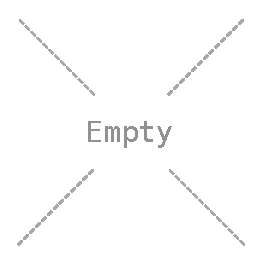
\includegraphics[height=\fgh]{empty.eps}
    }

    \mycaption{fig:eval-baseline}{Baseline I/O performance}{Median sequential
    and random I/O baseline as discussed in \cref{subsec:eval-baseline}.}
\end{figure}


\Cref{fig:eval-baseline} shows the baseline tradeoff between trade score
(x-axis; see also \cref{subsec:des-discussion}) and median normalized latency
(y-axis) of different crypts for our sequential and random I/O workloads
(sequential is shown). Trends for median hold when looking at tail latencies as
well. Each line represents one workload: 4KB, 512KB, 5MB, and 40MB respectively
(see legend). Each symbol represents one of our crypts: ChaCha8 (C8), ChaCha20
(C20), Freestyle Fast (FF), Freestyle Balanced (FB), and Freestyle Strong (FS).
Of these crypts, those with higher trade scores resulted in higher overall
latency and increased energy use for I/O operations. The relationship between
these concerns is not linear across crypts, however, which exposes a rich
tradeoff space.

Besides the 4KB workload, the shape of each workload follows a similar trend,
hence we will focus on 40MB and 4KB workloads here. Due to the overhead of
metadata management and the fast completion time of the 4KB workloads (\ie
little time for amortization of overhead), C8 and C20 take longer to complete
than FF. This advantage is not enough to make FB or Secure workloads complete
faster than the ChaCha variants, however.

Though C8 is faster than C20, there is some variability in our timing setup when
capturing extremely fast events occurring close together in time. This is why C8
sometimes appears with higher latency than C20 for normalized 4KB workloads. C8
is not slower than C20.


% =======================================================
\subsection{Heterogeneous FDE Performance}\label{subsec:eval-flexible}

\def \hmina {\hspace{-0.1in}}
\def \hminb {\hspace{-0.2in}}

\def \fgw {2in}
\def \fgh {1in}

% \begin{floatingfigure}[r]{2in}  (and \end{..})

\begin{figure}[t]
    \centerline{
        % \hmina
        {\begin{tikzpicture}[baseline]

    \pgfmathsetmacro{\ymax}{1.1} % set the maximum y value
    \pgfmathsetmacro{\ymaxbreak}{1.2} % set the y value at which overflow is drawn

    \begin{groupplot}[
        group style={
            group size=2 by 2,
            xlabels at=edge bottom,
            ylabels at=edge left,
            xticklabels at=edge bottom,
            yticklabels at=edge left,
            vertical sep=25pt,
            horizontal sep=15pt,
        },
        %axis x line*=bottom,
        height=3cm,
        width=\textwidth/4,
        tick align=outside,
        tick pos=bottom, % make sure ticks only appear at the bottom and left axes
        title style={yshift=-1.5ex},
        tick style={ black },
        y tick label style={ /pgf/number format/fixed, /pgf/number format/precision=0 },
        grid style={ dotted, gray },
        scatter,
        point meta=explicit symbolic,
        scatter/classes={
            c8={mark=square*},
            c20={mark=triangle*},
            ff={mark=diamond*},
            fb={mark=pentagon*},
            fs={mark=otimes}
        },
        %every node near coord/.append style={font=\tiny},
        %
        % magic to make the numbers appear above the overly long bars:
        % visualization depends on={rawy \as \rawy}, % save original y values
        % restrict y to domain*={ % now clip/restrict any y value to ymax
        %     \pgfkeysvalueof{/pgfplots/ymin}:\ymaxbreak
        % },
        % after end axis/.code={ % draw squiggly line indicating break
        %     \draw [semithick, white, decoration={snake,amplitude=0.1mm,segment length=0.75mm,post length=0.375mm}, decorate] (rel axis cs:0,1.01) -- (rel axis cs:1,1.01);
        % },
        % nodes near coords={\color{.!75!black}\pgfmathprintnumber\rawy}, % print the original y values (darkened in case they are too light)...
        % nodes near coords greater equal only=\ymax, % ... but ONLY if they are >= ymax
        % clip=false, % allow clip to protrude beyond ymax
        % Custom stuff to edit per template
        %
        xlabel={\scriptsize Trade Score},
        xlabel near ticks,
        %xlabel shift={-1.5mm},
        xmin=0, xmax=4,
        xtick={ 0, 1, 2, 3, 4 },
        xticklabels={ 0,,, 1, \empty },
        %major x tick style=transparent,
        %enlarge x limits=0.2, % add some breathing room along the x axis's sides
        %
        ylabel={\scriptsize Latency (norm)},
        ylabel near ticks,
        ylabel shift={-1.5mm},
        ymajorgrids=true,
        ymin=0, ymax=\ymax,
        ytick={ 0, 1, \ymax },
        yticklabels={ 0, 1, \empty },
        %yticklabels={ 0, 0.5, 1.5, 2 },
        % extra y ticks={1},
        % extra y tick style={grid=major, grid style={dashed, black}},
        % extra y tick label={\empty},
        %bar width=4.5pt, % change size of bars
        %
        legend cell align=left,
        legend style={ column sep=1ex },
        legend entries={
            {\scriptsize Baseline},
            {\scriptsize Ratios},
            {\scriptsize },
            {\scriptsize },
            {\scriptsize },
            {\scriptsize C8},
            {\scriptsize C20},
            {\scriptsize FF},
            {\scriptsize FB},
            {\scriptsize FS}
        },
        legend style={
            draw=none,
            legend columns=5,
            at={(1.0,1.35)},
            anchor=south,
        },
    ]
        \nextgroupplot[title={\footnotesize Sequential 40M Reads}]
            \addlegendimage{no markers,red}
            \addlegendimage{mark=otimes*,only marks,black}
            \addlegendimage{only marks,mark=square*,white}
            \addlegendimage{only marks,mark=square*,white}
            \addlegendimage{only marks,mark=square*,white}
            \addlegendimage{only marks,mark=square*,red}
            \addlegendimage{only marks,mark=triangle*,red}
            \addlegendimage{only marks,mark=diamond*,red}
            \addlegendimage{only marks,mark=pentagon*,red}
            \addlegendimage{only marks,mark=otimes,red}
            \addplot [thick, red] table [
                meta=cipher,
                x=score,
                y=latency,
                discard if symbol not={iop}{40m-r},
                discard if number not={ratio}{0},
                discard if symbol not={order}{seq},
                col sep=space,
            ] {data/tradeoff-forward.dat};
            \addplot [only marks] table [
                x=score,
                y=latency,
                discard if symbol not={iop}{40m-r},
                discard if number not={ratio}{1},
                discard if symbol not={order}{seq},
                col sep=space
            ] {data/tradeoff-forward.dat};
            \addplot [only marks] table [
                x=score,
                y=latency,
                discard if symbol not={iop}{40m-r},
                discard if number not={ratio}{2},
                discard if symbol not={order}{seq},
                col sep=space
            ] {data/tradeoff-forward.dat};
            \addplot [only marks] table [
                x=score,
                y=latency,
                discard if symbol not={iop}{40m-r},
                discard if number not={ratio}{3},
                discard if symbol not={order}{seq},
                col sep=space
            ] {data/tradeoff-forward.dat};
        \nextgroupplot[legend to name={throwaway5}, title={\footnotesize Sequential 40M Writes}]
            \addplot [thick, red] table [
                meta=cipher,
                x=score,
                y=latency,
                discard if symbol not={iop}{40m-w},
                discard if number not={ratio}{0},
                discard if symbol not={order}{seq},
                col sep=space,
            ] {data/tradeoff-forward.dat};
            \addplot [only marks] table [
                x=score,
                y=latency,
                discard if symbol not={iop}{40m-w},
                discard if number not={ratio}{1},
                discard if symbol not={order}{seq},
                col sep=space
            ] {data/tradeoff-forward.dat};
            \addplot [only marks] table [
                x=score,
                y=latency,
                discard if symbol not={iop}{40m-w},
                discard if number not={ratio}{2},
                discard if symbol not={order}{seq},
                col sep=space
            ] {data/tradeoff-forward.dat};
            \addplot [only marks] table [
                x=score,
                y=latency,
                discard if symbol not={iop}{40m-w},
                discard if number not={ratio}{3},
                discard if symbol not={order}{seq},
                col sep=space
            ] {data/tradeoff-forward.dat};
        \nextgroupplot[legend to name={throwaway4}, title={\footnotesize Sequential 4K Reads}]
            \addplot [thick, red] table [
                meta=cipher,
                x=score,
                y=latency,
                discard if symbol not={iop}{4k-r},
                discard if number not={ratio}{0},
                discard if symbol not={order}{seq},
                col sep=space,
            ] {data/tradeoff-forward.dat};
            \addplot [only marks] table [
                x=score,
                y=latency,
                discard if symbol not={iop}{4k-r},
                discard if number not={ratio}{1},
                discard if symbol not={order}{seq},
                col sep=space
            ] {data/tradeoff-forward.dat};
            \addplot [only marks] table [
                x=score,
                y=latency,
                discard if symbol not={iop}{4k-r},
                discard if number not={ratio}{2},
                discard if symbol not={order}{seq},
                col sep=space
            ] {data/tradeoff-forward.dat};
            \addplot [only marks] table [
                x=score,
                y=latency,
                discard if symbol not={iop}{4k-r},
                discard if number not={ratio}{3},
                discard if symbol not={order}{seq},
                col sep=space
            ] {data/tradeoff-forward.dat};
        \nextgroupplot[legend to name={throwaway6}, title={\footnotesize Sequential 4K Writes}]
            \addplot [thick, red] table [
                meta=cipher,
                x=score,
                y=latency,
                discard if symbol not={iop}{4k-w},
                discard if number not={ratio}{0},
                discard if symbol not={order}{seq},
                col sep=space,
            ] {data/tradeoff-forward.dat};
            \addplot [only marks] table [
                x=score,
                y=latency,
                discard if symbol not={iop}{4k-w},
                discard if number not={ratio}{1},
                discard if symbol not={order}{seq},
                col sep=space
            ] {data/tradeoff-forward.dat};
            \addplot [only marks] table [
                x=score,
                y=latency,
                discard if symbol not={iop}{4k-w},
                discard if number not={ratio}{2},
                discard if symbol not={order}{seq},
                col sep=space
            ] {data/tradeoff-forward.dat};
            \addplot [only marks] table [
                x=score,
                y=latency,
                discard if symbol not={iop}{4k-w},
                discard if number not={ratio}{3},
                discard if symbol not={order}{seq},
                col sep=space
            ] {data/tradeoff-forward.dat};
    \end{groupplot}
\end{tikzpicture}%
}
        % \hminb
        %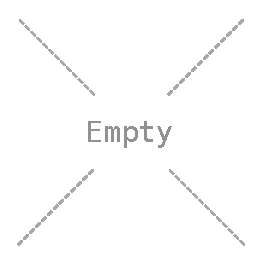
\includegraphics[height=\fgh]{empty.eps}
    }

    \mycaption{fig:eval-forward}{Forward I/O performance}{Median sequential I/O
    compared to baseline. Each cluster of 3 dots between configurations
    represents the 7:3, 5:5, and 3:7 ratios as discussed in
    \cref{subsec:eval-flexible}. Distance from baseline represents overhead.}
\end{figure}


\Cref{fig:eval-forward} shows the tradeoff between trade score (x-axis; see also
\cref{subsec:des-discussion}) and median normalized latency (y-axis) of
different crypts for our sequential and random I/O workloads (sequential is
shown) using Forward switching. After a certain number of write-read operations
using the primary crypt, a switch is initiated and \sys begins using the
secondary crypt for I/O. For each of the four pairs of crypts in the figure
(primary+secondary: C8+C20, C20+FF, FF+FB, FB+FS), this is repeated three times:
once at every ratio point {\em between} our baseline crypt measurements
(\ie{7:3, 5:5, and 3:7 described above}). Ratio points above baseline measure
overhead.

\def \hmina {\hspace{-0.1in}}
\def \hminb {\hspace{-0.2in}}

\def \fgw {2in}
\def \fgh {1in}

% \begin{floatingfigure}[r]{2in}  (and \end{..})

\begin{figure}[t]
    \centerline{
        % \hmina
        % {\input{data/eval-ms}}
        % \hminb
        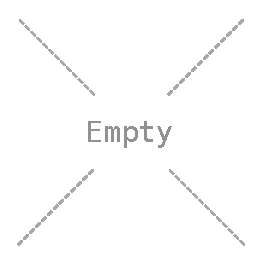
\includegraphics[height=\fgh]{empty.eps}
    }

    \mycaption{fig:eval-ms}{Mirrored and Selective I/O performance}{Median
    sequential and random I/O compared to baseline. Each cluster of 3 dots
    between configurations represents the 7:3, 5:5, and 3:7 ratios as discussed
    in \cref{subsec:eval-dynamic}.}
\end{figure}


The point of this experiment is to determine if \sys can switch the encryption
efficiently enough to support heterogeneous FDE---that is, contiguous nuggets
encrypted with different crypts---without devastating performance. For the 40MB,
5MB, and 512KB workloads (40MB is shown), we see that overhead is low,
demonstrating that with heterogeneous FDE we can in fact achieve flexible
security/energy tradeoffs unachievable with prior work and all with minimal
overhead.

Again, due to the overhead of metadata management and fast completion time of
the workloads, C8 and C20 take longer to complete than FF for 4KB reads. We also
see very high latency for ratios between FF and FS crypts. This is because
Freestyle is non-length-preserving, so extra operations must be performed on
every write, and the algorithm itself is generally much slower than the ChaCha
variants.

\Cref{fig:eval-ms} shows the performance of the Mirrored and Selective models vs
baseline with the same configuration of ratios as \cref{fig:eval-forward}.

For the 40MB, 5MB, and 512KB workloads (40MB is shown), we see that Mirrored and
Selective {\em read} workloads and the Selective {\em write} workload have
similar latency overhead to the Forward model experiments. This makes sense, as
most of the overhead for Selective and Mirrored reads is determining which part
of the drive to commit data to. The same applies to Selective writes. For the
4KB Mirrored and Selective {\em read} workloads and the Selective {\em write}
workload, we see behavior similar to that in \cref{fig:eval-forward}, as
expected.

Mirrored writes across all workloads are slow. This is to be expected since
writes are being duplicated. This overhead is highest for the 4KB Mirrored write
workload.


% =======================================================
\subsection{Summary Discussion}\label{subsec:eval-overhead}

We calculate that Forward switching has average latency overhead at 0.08x/0.10x
(read/write) for 40MB, 5MB and 512KB workloads compared to baseline I/O,
demonstrating \sys's amortization of switching costs. Average overhead is
0.38x/0.44x (read/write) for 4KB workloads, where \sys is unable to amortize
cost. Similarly, we calculate that Selective switching has average overhead at
\TODO{0x/Zx} (read/write) for 40MB, 5MB and 512KB workloads compared to baseline
I/O. Average overhead is \TODO{Yx/Zx} (read/write) for 4KB workloads. Finally,
we calculate that Mirrored switching has average overhead at \TODO{Yx/Zx}
(read/write) for 40MB, 5MB and 512KB workloads compared to baseline I/O, with
high write latency due to mirroring. Average overhead is \TODO{Yx/Zx}
(read/write) for 4KB workloads.

In summary, these results show that \sys enables a wide range of performance and
security tradeoffs unachievable with prior work. This useful feature comes at a
cost of at most \TODO{Yx/Zx} increased read/write overhead (excluding Mirrored)
compared to existing FDE approaches like StrongBox, and at the cost of reduced
performance for very small workloads. We conclude that any FDE workload
dominated by I/Os larger than 4KB would benefit from the increased flexibility
of \sys and heterogeneous FDE.
